%\begin{figure}
%  \centering
  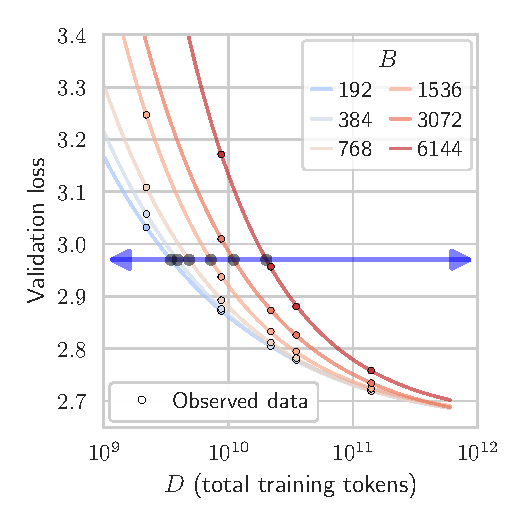
\includegraphics[trim={0.3cm 0.4cm 0.3cm 0.3cm}, clip, width=\linewidth]{pdffigs/241005.fitted_scale_law.gbs=multi.111M.l=2.97.pdf}
  %Scaling laws in $D$ for computing $\cbs$} (111M
  %scale): after training with different batch sizes, $B$, and
  %dataset sizes, $D$ (indicated by points on curves), we fit
  \caption{(111M): \textbf{Fitted $B$-specific power laws},
  $L_B(D)$, for inferring steps to reach target loss $\lhat$ (arrowed
  blue line).\label{fig:cbs_fitting}}
%
%    .  We can then
%    compute the amount of data needed to reach any target loss
  %    (arrowed line) for each batch size via $L_B^{-1}(D)$;
%  this
%    provides the points over which we fit \cref{eq:tradeoff} and
%    determine $\cbs$. .}}
%\end{figure}

    
